% !TEX root = ../main.tex
% Хавсралт Ж

\chapter{Тайлбарлах чадварын үр дүн}
\label{AppendixG}
\pagecolor{white}

(Зургуудыг \texttt{appendix\_scripts/gen\_G\_explainability.py} script-ээр үүсгэнэ.)

\section*{Grad-CAM}

Grad-CAM-ийн үр дүнгээс харахад ангиллын загвар нь шийдвэр гаргахдаа хугарлын бүсэд төвлөрч байгааг харуулсан. Зураг~\ref{fig:appG_gradcam1}--\ref{fig:appG_gradcam5}-д Grad-CAM-ийн жишээнүүдийг үзүүлэв.

\begin{figure}[H]
    \centering
    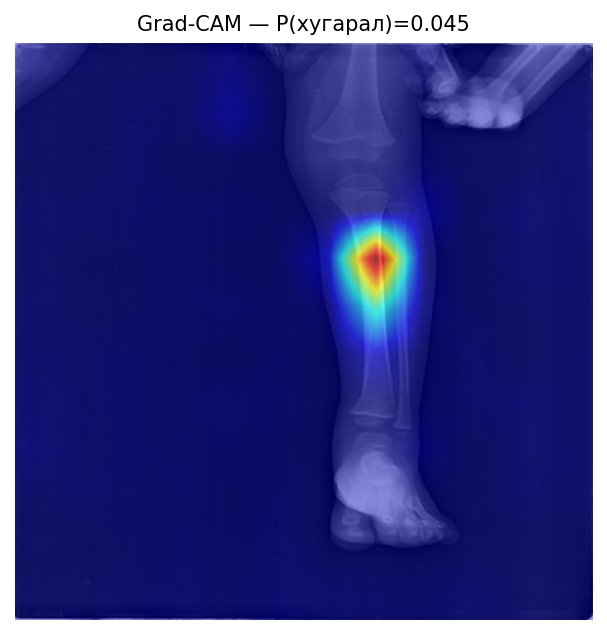
\includegraphics[width=0.43\textwidth,height=0.45\textheight,keepaspectratio]{Figures/appx_g_gradcam_1.png}
    \figcaption{Grad-CAM жишээ 1}{Grad-CAM жишээ 1}
    \label{fig:appG_gradcam1}
\end{figure}

\begin{figure}[H]
    \centering
    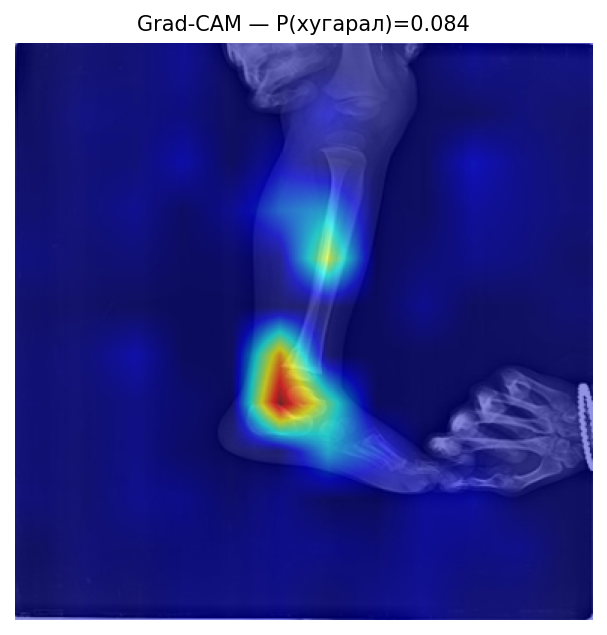
\includegraphics[width=0.43\textwidth,height=0.45\textheight,keepaspectratio]{Figures/appx_g_gradcam_2.png}
    \figcaption{Grad-CAM жишээ 2}{Grad-CAM жишээ 2}
    \label{fig:appG_gradcam2}
\end{figure}

\begin{figure}[H]
    \centering
    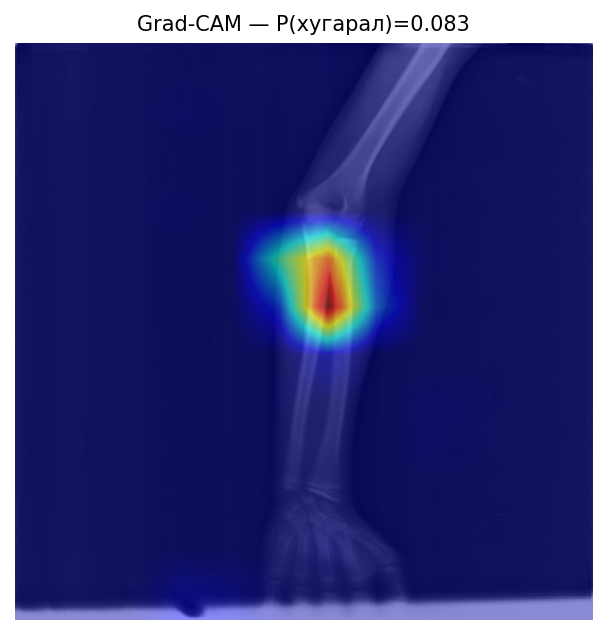
\includegraphics[width=0.43\textwidth,height=0.45\textheight,keepaspectratio]{Figures/appx_g_gradcam_3.png}
    \figcaption{Grad-CAM жишээ 3}{Grad-CAM жишээ 3}
    \label{fig:appG_gradcam3}
\end{figure}

\begin{figure}[H]
    \centering
    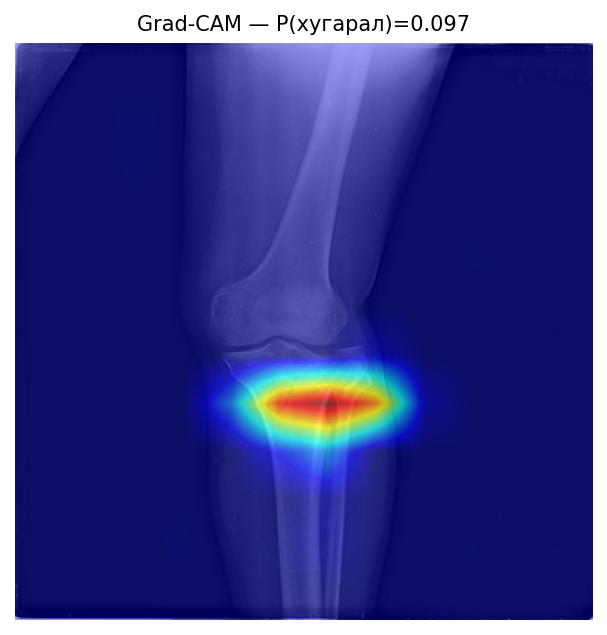
\includegraphics[width=0.43\textwidth,height=0.45\textheight,keepaspectratio]{Figures/appx_g_gradcam_4.png}
    \figcaption{Grad-CAM жишээ 4}{Grad-CAM жишээ 4}
    \label{fig:appG_gradcam4}
\end{figure}

\begin{figure}[H]
    \centering
    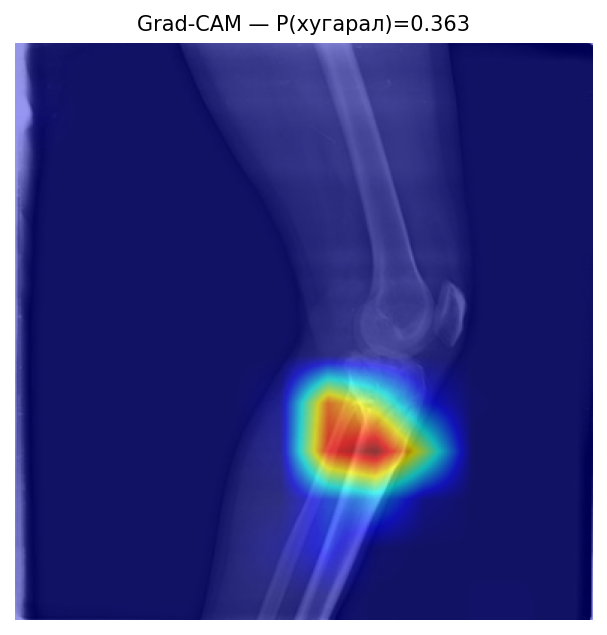
\includegraphics[width=0.43\textwidth,height=0.45\textheight,keepaspectratio]{Figures/appx_g_gradcam_5.png}
    \figcaption{Grad-CAM жишээ 5}{Grad-CAM жишээ 5}
    \label{fig:appG_gradcam5}
\end{figure}

\section*{SHAP}

SHAP шинжилгээ нь эдгэрэлтийн үнэлгээнд нөлөөлж буй гол хүчин зүйлүүдийг тайлбарлах боломж олгосон.

\begin{figure}[H]
    \centering
    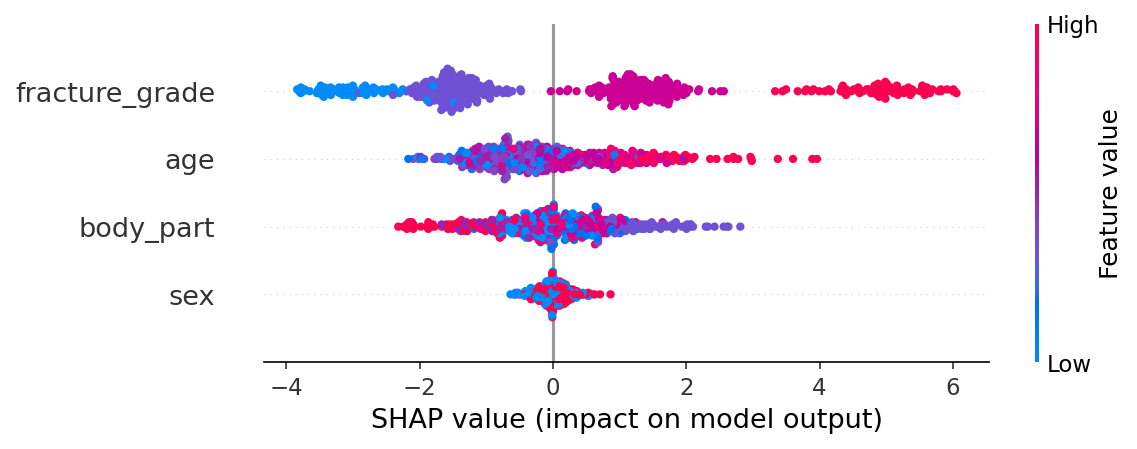
\includegraphics[width=0.66\textwidth,height=0.36\textheight,keepaspectratio]{Figures/appx_g_shap_summary.png}
    \figcaption{SHAP Summary Plot}{SHAP Summary Plot}
    \label{fig:appG_shap_summary}
\end{figure}

\begin{figure}[H]
    \centering
    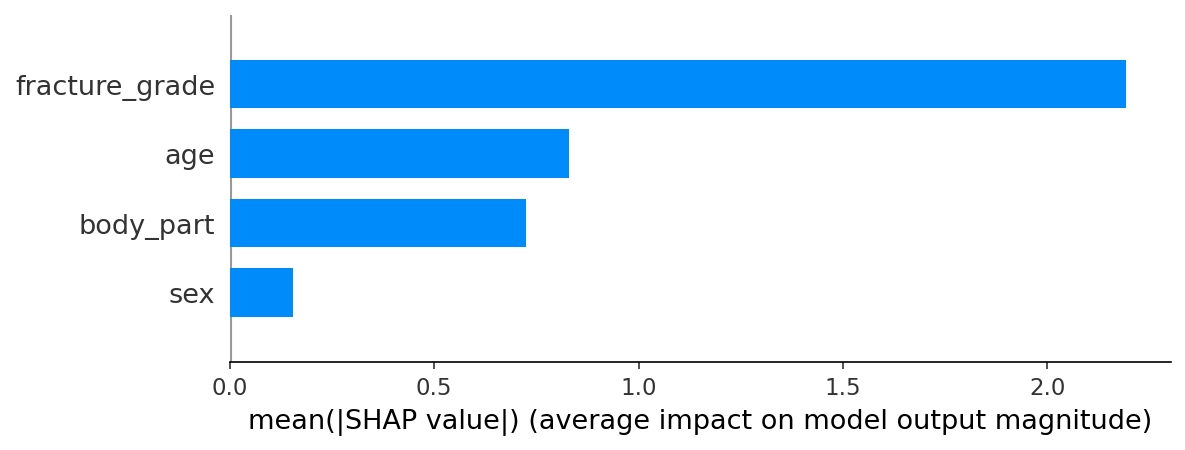
\includegraphics[width=0.66\textwidth,height=0.36\textheight,keepaspectratio]{Figures/appx_g_shap_feat.png}
    \figcaption{Feature Importance Plot}{Feature Importance Plot}
    \label{fig:appG_shap_feat}
\end{figure}
